
\begin{document}

\chapter{Methodology}

\label{chapter:methodology}

\section{Dynamic Obstacles}

As a main component of this work, dynamic obstacles needed to be designed such
that one could quantify their trajectories, initial configurations, and their
level of uncertainty. This section introduces the definition of a dynamic
obstacle used throughout this work along with how it is represented to the
planner and its simulated \& predicted equations of motion.

\subsection{Definition}

A dynamic obstacle is defined as a 5-tuple, $a = (I, \dot{\zeta},
\epsilon, \xi, T)$ where $I$ is the initial configuration of the obstacle,
$\dot{\zeta}$ is a function, $\dot{\zeta}: \mathbb{R}^+ \rightarrow
\mathbb{R}^2$, representing the velocity of the obstacle, $\epsilon$ is used to
define a random variable $\rho \sim \mathcal{U}(-\epsilon, \epsilon)$ that is
injects noise into an obstacle's trajectory shown in Eq.~\ref{eq:obs_observed}
where $\mathcal{U}$ is a uniform distribution, $\xi$ is the current
configuration used for prediction, and $T$ is the time that the obstacle was in
configuration $\xi$.  The variables $\xi$ and $T$ are dynamic variables and are
updated throughout the execution of the algorithm and are used to determine
when it is appropriate for the algorithm replan and find a new path through the
environment using more up to date information. This is explained in
Sec.~\ref{sec:design_planner}. The variables $\xi$ and $T$ are initially set to
$I$ and $0$ respectively.

\subsection{Cost Function}

\label{sec:cost}

Unlike in the previous work, dynamic obstacles are represented by cost
distributions that resemble probability density functions. The difference being
is that these cost distributions do not have a unit integral. These cost
distributions are used to describe where the obstacle is going to be in within
a time interval and can be generated by a third party system, such as a motion
capture system. There is an assumption that for a given interval, $\mathcal{T}
= [t_0, t_m]$, the highest cost with the smallest uncertainty will be at $t =
t_0$ and the lowest cost with the highest uncertainty will be at $t = t_m$.
Under this assumption, the cost function models how the obstacle may diverge
from its current trajectory as time increases. With these assumptions, the cost
function, $P_a: \mathbb{R}^2 \times (\mathbb{R}^+)^2 \rightarrow
\mathbb{R}$, represents represents the cost surface for a given
obstacle within a given time interval. Eq.~\ref{eq:singleprob} formally defines
the cost function for a single obstacle.

% Single agent PDF

\begin{equation}
    P_a(x, y, t_0, t_m) = \int^{t_m}_{t_0}
    \mathcal{N}(\zeta_a(t), \alpha \cdot (t - t_0)^2 + \beta, x, y) \cdot
    (t_m - t)^{\gamma} \,\mathrm{d}t
    \label{eq:singleprob}
\end{equation}

In Eq.~\ref{eq:singleprob}, $\mathcal{N}(\mu, \sigma^2, x, y)$ is the
evaluation of a 3D normal distribution centered at $(\mu_x, \mu_y)$ with a
variance of $\sigma^2$ at $(x, y)$. Fig.~\ref{fig:normal_3d} shows an example
of $\mathcal{N}$. This equation models how the uncertainty of obstacle
trajectory prediction increases over time by increasing the standard deviation
of the Gaussian distribution as the time increases.  Likewise, this function
multiplies the Gaussian distribution by a factor of $(t_m - t)^{\gamma}$ where
$\gamma \geq 1$ which gives higher costs to times closer to $t_0$.

\begin{figure}[h!]
    \centering
    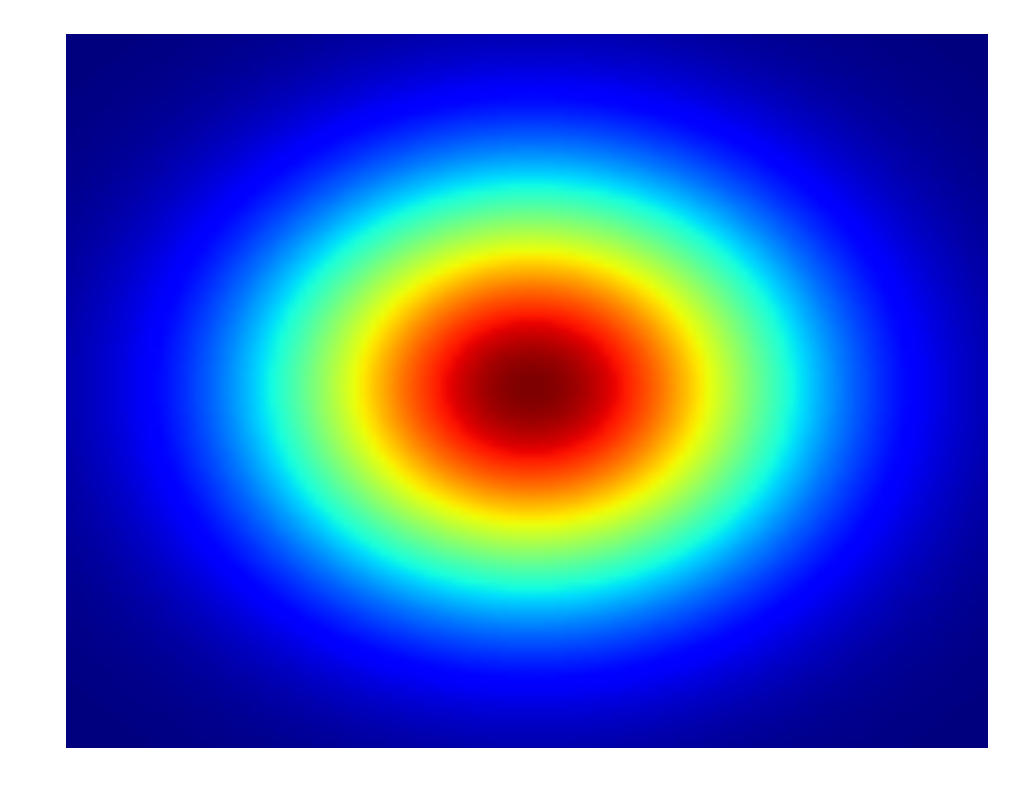
\includegraphics[width=0.60\linewidth]{figs/normal_3d}
    \caption{}
    \label{fig:normal_3d}
\end{figure}

A cost function is also needed that can incorporate the cost distributions for
multiple dynamic obstacles within the environment. The cost function used in
this work, $P: \mathbb{R}^2 \times (\mathbb{R}^+)^2 \times \mathcal{A}
\rightarrow \mathbb{R}$ where $\mathcal{A}$ is the set of all possible sets of
dynamic obstacles, calculates the average cost at a point $(x, y)$ within a
given time interval for a given set of agents. This is shown formally in
Eq.~\ref{eq:prob}.

% Multiple agent PDF

\begin{equation}
    P(x, y, t_0, t_m, A) = \frac{\mathlarger{\sum_{a \in A} P_a(x, y, t_0,
    t_m)}}{|A|}
    \label{eq:prob}
\end{equation}

An example of how $P$ changes over time is shown in Fig.~\ref{fig:agent_cost}.
In that example, two dynamic obstacles are placed in the scene and given
sinusoidal velocities. In this example the time interval, $\delta t$, is kept
constant throughout the simulation, i.e. $t_m = t_0 + \delta t$, for all $t_0
\in [0, T - \delta t]$ where $T$ is the length of the simulation. Since the
velocity does not remain constant in the example, the cost distribution
elongates an shrinks based on the acceleration of the obstacle. For instance,
in the first and last images in Fig.~\ref{fig:agent_cost}, the cost is
contained to a small area due to the velocity equations of the obstacles being
at their minimum and in the fourth image,the cost is more spread out through
the environment because the velocity is at its maximum.

\begin{figure}[h!]

    \centering

    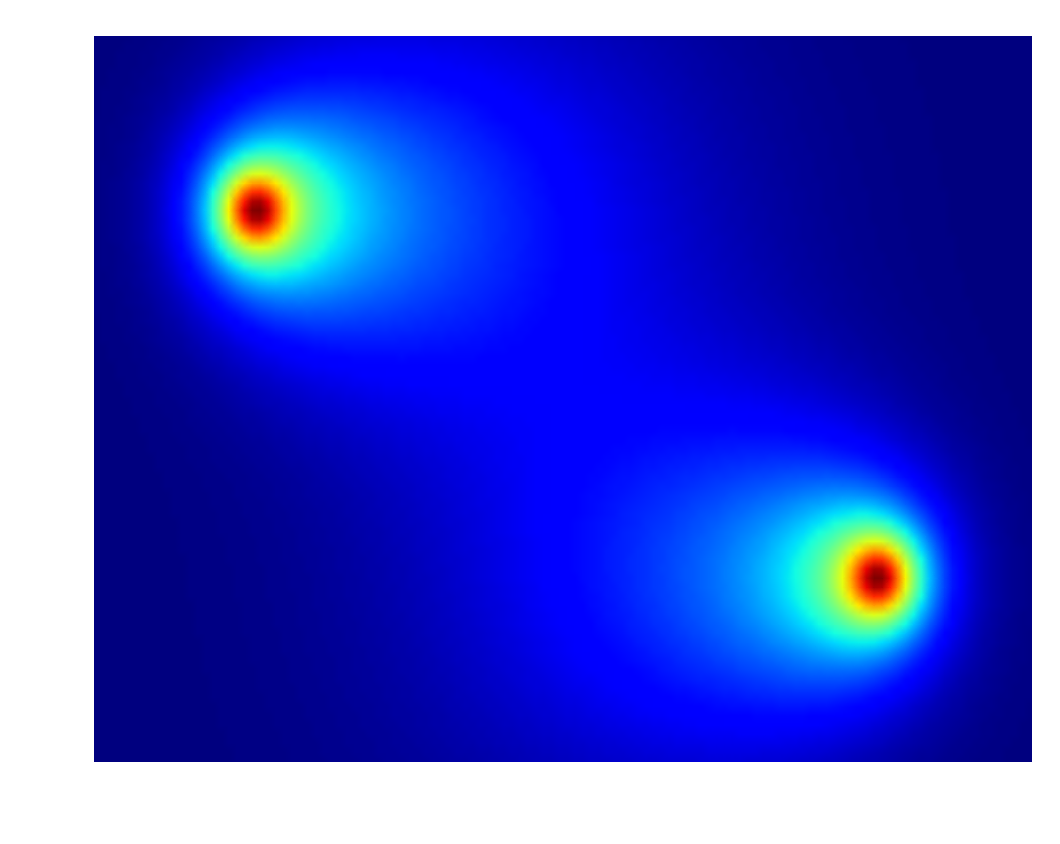
\includegraphics[width=0.24\linewidth]{figs/agent_1}
    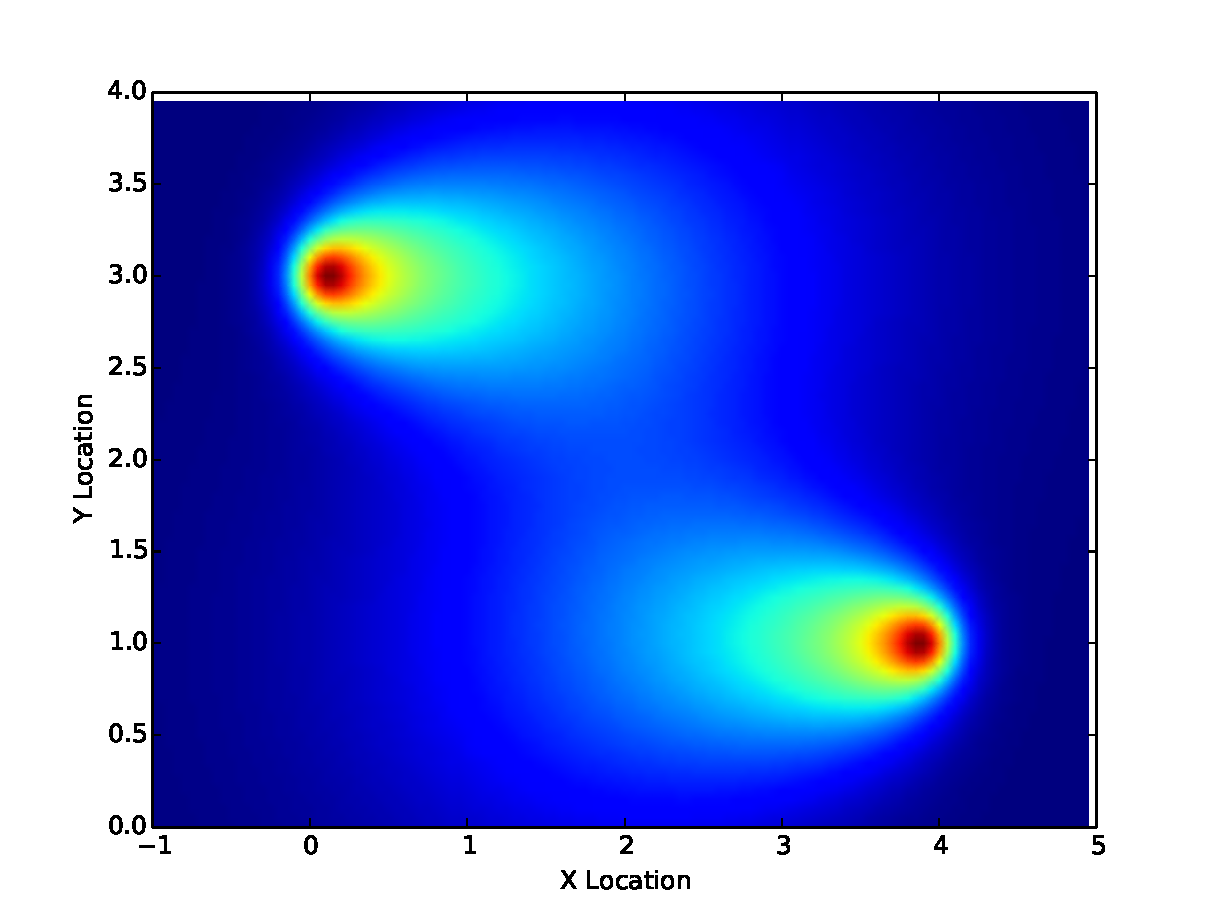
\includegraphics[width=0.24\linewidth]{figs/agent_2}
    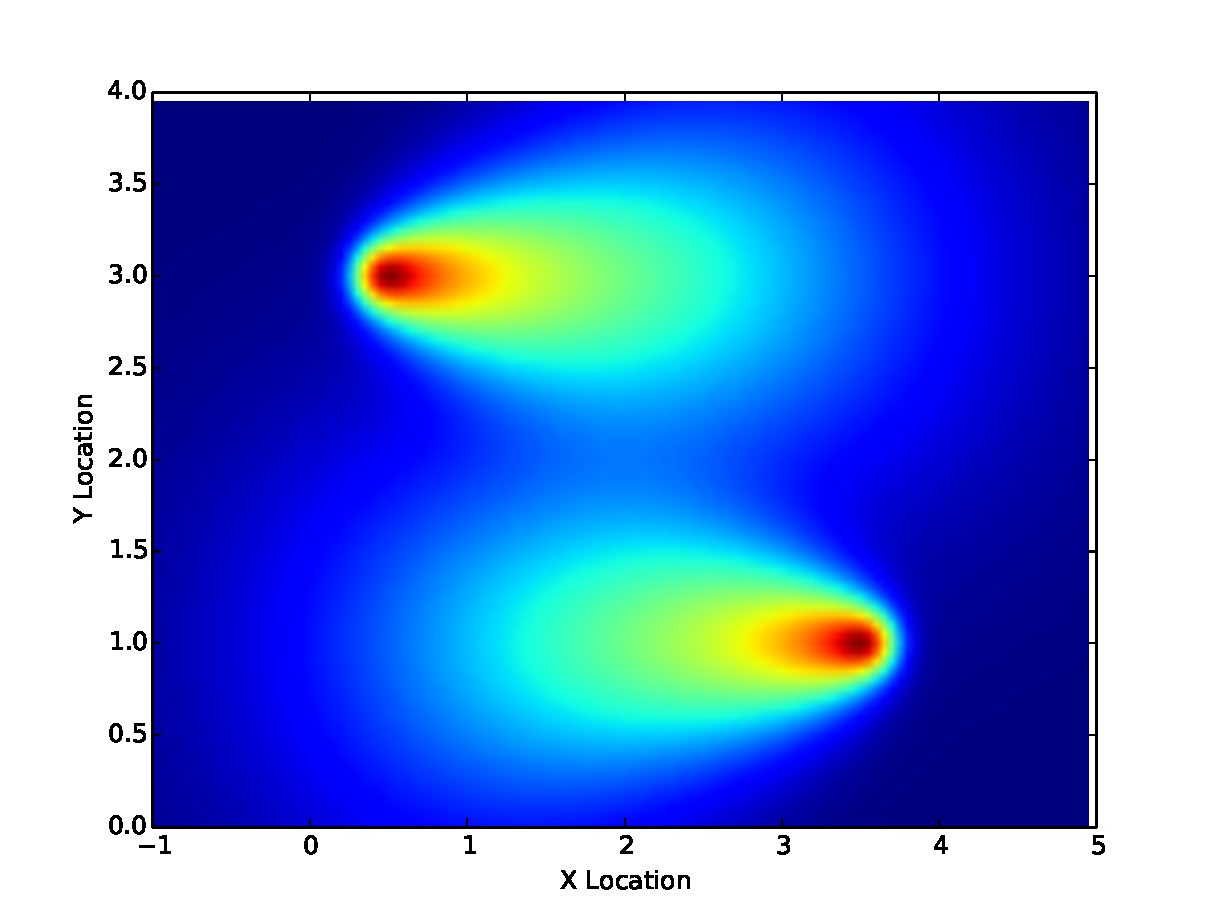
\includegraphics[width=0.24\linewidth]{figs/agent_3}
    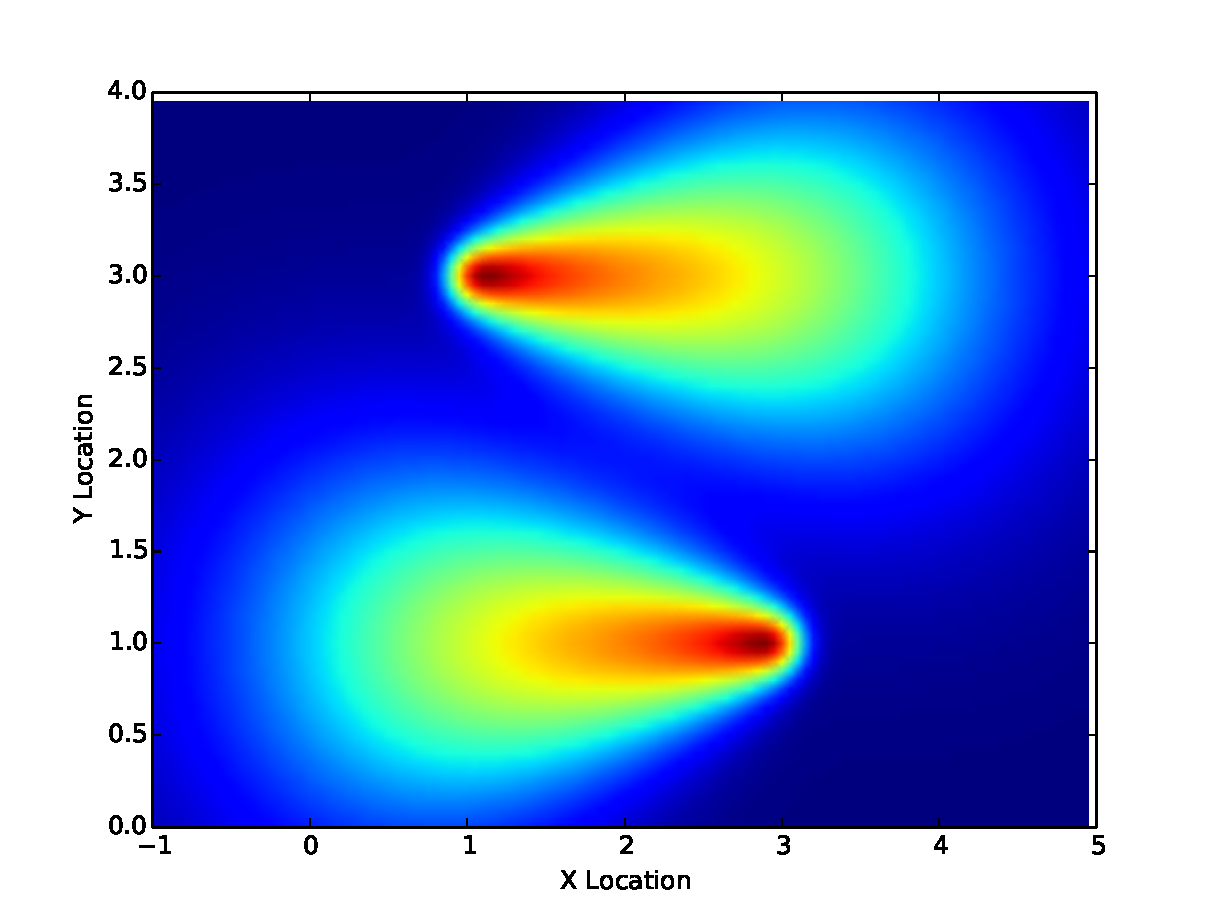
\includegraphics[width=0.24\linewidth]{figs/agent_4} \\
    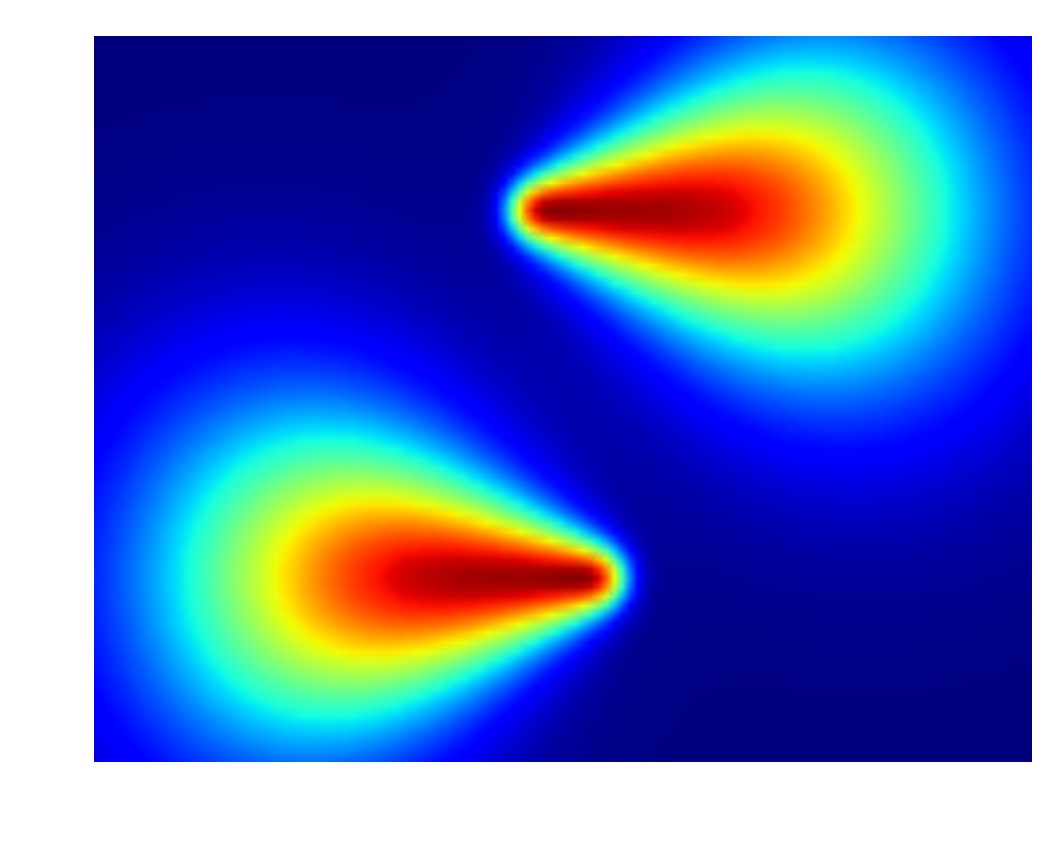
\includegraphics[width=0.24\linewidth]{figs/agent_5}
    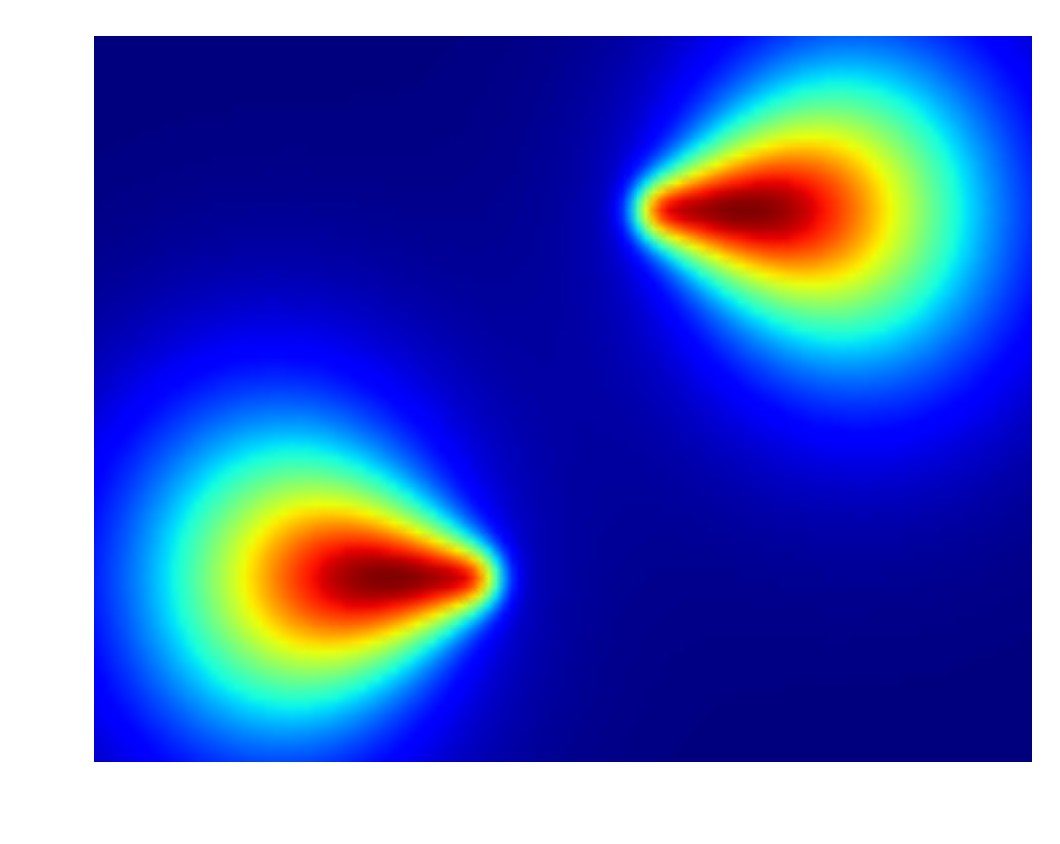
\includegraphics[width=0.24\linewidth]{figs/agent_6}
    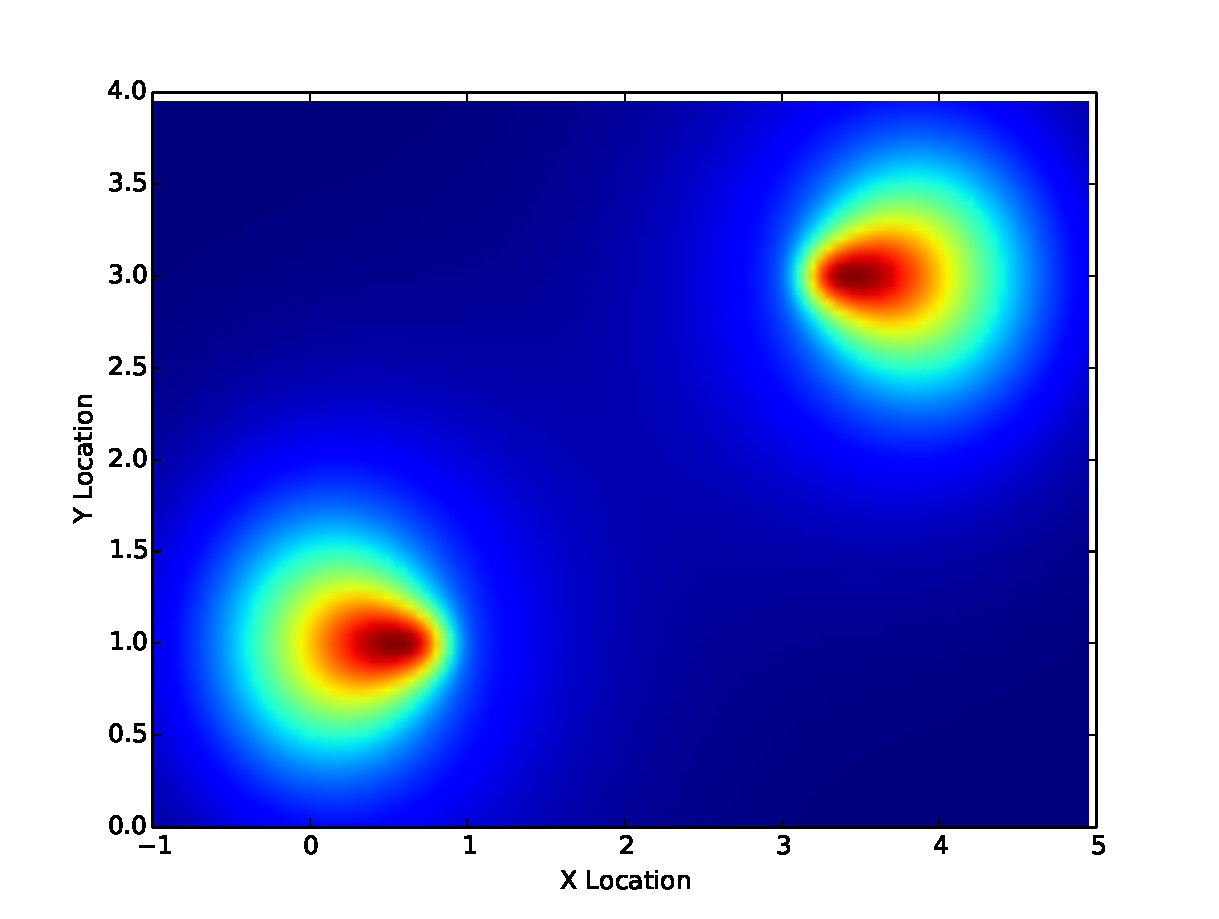
\includegraphics[width=0.24\linewidth]{figs/agent_7}
    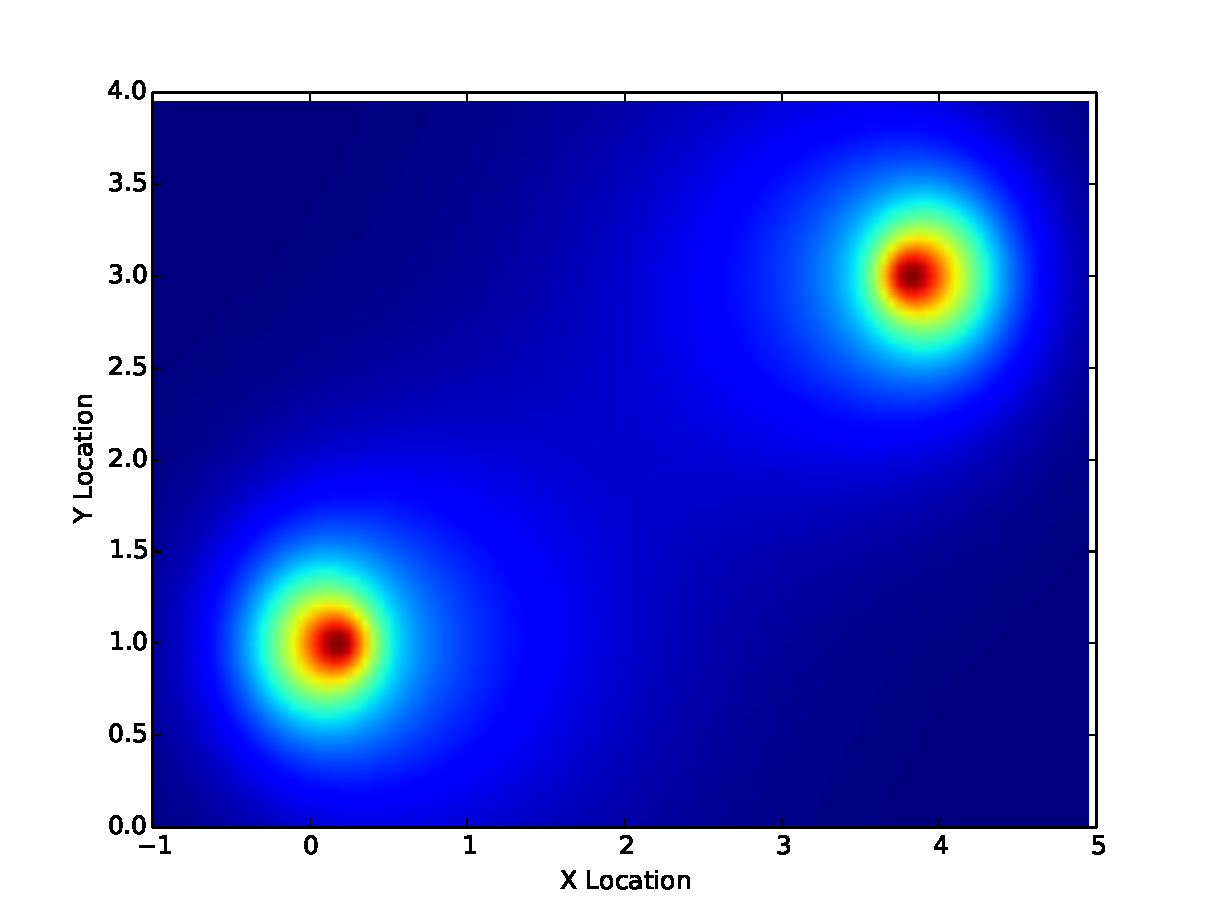
\includegraphics[width=0.24\linewidth]{figs/agent_8}

    \caption{Cost distributions indicating the likelihood that an agent will be
    at a certain location within a given time interval.  These figures show how
this distribution changes over time (left to right, top to bottom)}

    \label{fig:agent_cost}

\end{figure}

\subsection{Equations of Motion}

The motion of a dynamic obstacle is defined by the velocity equation, the
initial configuration, the amount of uncertainty. Defining the obstacle's
trajectory in terms of its velocity makes it easier to model when creating
scenes. The equation of motion for the dynamic obstacle is shown in
Eq.~\ref{eq:obs_pred}.

\begin{equation}
    \zeta_a(t) =
        \begin{cases}
            \xi_a + \mathlarger{\int_{T_a}^{t}} \dot{\zeta_a}(\lambda) \,
            \mathrm{d}\lambda
            & \text{if } t \geq T_a \\
            \tilde{\zeta_a}(t) & \text{if } t < T_a
        \end{cases}
    \label{eq:obs_pred}
\end{equation}

In Eq.~\ref{eq:obs_pred}, $\tilde{\zeta_a}$ represents the observed trajectory
of the obstacle whereas $\zeta_a$ corresponds to the predicted trajectory of
the obstacle. This disambiguation is needed because the planner needs to be
able to extrapolate the future movements of a dynamic obstacle. The variables,
$\xi_a$ and $T_a$ are dynamically updated when the planner replans and are
initially set to $I_a$ and $0$ respectively. The need for this and how it is
designed will be discussed in Sec.~\ref{sec:design_planner}

For the experiments, the motion of the obstacles are simulated by adding a
random variable, $\rho \sim \mathcal{U}(-\epsilon, \epsilon)$ to the trajectory
during the integration of the velocity equation. This form of stochasticity
allows the obstacle to diverge from its specified trajectory whilst maintaining
the same velocity equation. This means that the obstacle will not exhibit
random motion around its specified path, but rather is able to diverge
completely. Also, by adding the random variable to the velocity equation during
integration, the obstacle will not "jump" to a new location, but will gradually
diverge and because it is analogous to the way the random variable was used
during the numerical integration in the code. The definition of
$\tilde{\zeta_a}$ is shown in Eq.~\ref{eq:obs_observed}.  For this equation, it
is assumed that the function only computes a value for any given time value,
$t$, only once.

\begin{equation}
    \tilde{\zeta_a}(t) = I_a + \int_{0}^{t} \dot{\zeta_a}(\lambda)
    + \rho \, \mathrm{d}\lambda
    \label{eq:obs_observed}
\end{equation}

The motion of a dynamic obstacle is described by it's velocity and a starting
location in order for the planner to be able to continue to predict an
obstacle's motion when it diverges from its current path. If the obstacle's
motion was described by parametric equations of it's position, it would not be
possible to continue to predict where it is going to move once it is no longer
following its prescribed path.

\section{Planning Algorithm}

\label{sec:design_planner}

% Graph cost function

\begin{equation}
    C(i, j, t_0, t_m, A) = \int^1_0 \exp{\Big(
        P(x(\lambda), y(\lambda), t_0, t_m, A) + 1 \Big)
    } \cdot ||i - j||_{2} \,\mathrm{d}\lambda
    \label{eq:cost}
\end{equation}

Where $x(\lambda) = (j_x - i_x) \cdot \lambda + i_x$ and $y(\lambda) = (j_y -
i_y) \cdot \lambda + i_y$ are the parametric equations of the line from $i$ to
$j$.


% Algorithm to generate a roadmap
\begin{algorithm}[ht]
    \caption{$\Function{Roadmap}(n, d, w, h, O)$}
    \algorithmicrequire{
        \\$n$: Maximum number of samples
        \\$d$: Maximum distance between neighbouring nodes
        \\$O$: Set of obstacles
    }
    \\\algorithmicensure{
        \\An unweighted graph of points describing the
        connectivity of the environment
    }
    \label{algo:prm}
    \begin{algorithmic}[1]
        \setcounter{ALC@line}{0}
        \vspace*{1mm}

        \FOR{$i = 1$ \TO $n$}
            \STATE $q \leftarrow \Function{RandomPoint2D}(w, h)$
            \IF{$\bigwedge_{o \in O} \neg \Function{Collision}(o, q)$}
                \STATE $V \leftarrow V \cup \{q\}$
            \ENDIF
        \ENDFOR

        \FORALL{$q_i \in V$}
            \FORALL{$q_j \in V$}
                \IF{$q_i \neq q_j \wedge ||q_i - q_j|| \leq d$}
                    \STATE $E \leftarrow E \cup \{(q_i, q_j)\}$
                    % \STATE $E \leftarrow E \cup \{(q_j, q_i)\}$
                \ENDIF
            \ENDFOR
        \ENDFOR
        \RETURN $(V,E)$
    \end{algorithmic}
\end{algorithm}

% Main algorithm to get the path
\begin{algorithm}[ht]
    \caption{$\Function{GetPath}(n, d, w, h, \delta, p, g, O, A, R)$}
    \algorithmicrequire{
        \\$n$: Maximum number of samples for the roadmap
        \\$d$: Maximum distance between neighbouring nodes in the roadmap
        \\$w$: Width of the scene
        \\$h$: Height of the scene
    }
    \\\algorithmicensure{}
    \label{algo:path}
    \begin{algorithmic}[1]
        \setcounter{ALC@line}{0}
        \STATE $(V, E) \leftarrow \Function{Roadmap}(n, d, w, h, O)$
        \STATE $\Pi \leftarrow \emptyset$
        \STATE $q \leftarrow p$
        \STATE $t \leftarrow 0$
        \WHILE {$||\Function{Back}(\Pi) - g||_2 > R$}
            \STATE $\pi \leftarrow \Function{SearchGraph}(V, E, R, A, q, g, t)$
            \FORALL {$(i, t') \in \pi$}
                \STATE $\Pi \leftarrow \Pi \cup \{i\}$
                \FORALL {$a \in A$}
                    \STATE $\Function{Step}(a)$
                \ENDFOR
                \IF {$\bigvee_{a \in A} ||\tilde{\zeta_a}(t') -
                    \zeta_a(t')|| > \delta$}
                    \FORALL {$a \in A$}
                        \STATE $\Function{Update}(\zeta_a, \tilde{\zeta_a})$
                    \ENDFOR
                    \STATE $q \leftarrow i$
                    \STATE $t \leftarrow t'$
                    \STATE $\textbf{break}$
                \ENDIF
            \ENDFOR
        \ENDWHILE
        \RETURN $\Pi$
    \end{algorithmic}
\end{algorithm}

% Algorithm to search the graph
\begin{algorithm}[ht]
    \caption{$\Function{SearchGraph}(V, E, R, A, p, g, T)$}
    % \algorithmicrequire{}
    % \\\algorithmicensure{}
    \label{algo:search}
    \begin{algorithmic}[1]
        \setcounter{ALC@line}{0}
        \vspace*{1mm}
        \STATE $Q \leftarrow \Function{PriorityQueue}()$
        \STATE $D \leftarrow \Function{Dictionary}()$
        \STATE $\mathcal{P} \leftarrow \Function{Dictionary}()$
        \STATE $\Function{Insert}(Q, p, T)$
        \WHILE {$\neg \Function{Empty}(Q)$}
            \STATE $(q, t) \leftarrow \Function{Pop}(Q)$
            \IF{$||q - g|| \leq R$}
                \RETURN $\Function{BacktrackPath}(p, g, \mathcal{P})$
            \ENDIF
            \STATE $S \leftarrow \emptyset$
            \STATE $N \leftarrow \Function{Neighbours}(V, E, q)$
            \FORALL {$n \in N$}
                \STATE $t' \leftarrow ||q - n|| / s + t$
                \STATE $\mathcal{P}_{(n, t')} \leftarrow (q, t)$
                \STATE $c \leftarrow \psi \cdot C(q, n, t, t', A) + \omega \cdot D_{\eta}$
                \STATE $D_{n} \leftarrow D_{n} + 1$
                \STATE $Q \leftarrow \Function{Insert}(Q, (n, t'), c)$
            \ENDFOR
        \ENDWHILE
    \end{algorithmic}
\end{algorithm}

% Given a parent dictionary, this returns the backtracked path
\begin{algorithm}[ht]
    \caption{$\Function{BacktrackPath}(p, g, \mathcal{P})$}
    % \algorithmicrequire{}
    % \\\algorithmicensure{}
    \label{algo:backtrack}
    \begin{algorithmic}[1]
        \setcounter{ALC@line}{0}
        \vspace*{1mm}
        \STATE $q \leftarrow g$
        \STATE $S \leftarrow \Function{Stack}()$
        \WHILE {$\mathcal{P}_q \neq p$}
            \STATE $S \leftarrow \Function{Push}(S, q)$
            \STATE $(q, t) \leftarrow \mathcal{P}_{q, t})$
        \ENDWHILE
        \STATE $S \leftarrow \Function{Push}(S, p)$
        \RETURN $S$
    \end{algorithmic}
\end{algorithm}

\end{document}
